%!TEX TS-program = xelatex

\documentclass[]{cv-class}
\usepackage{afterpage}
\usepackage{hyperref}
\usepackage{color}
\usepackage{xcolor}
\hypersetup{
    colorlinks=true,
    linkcolor=blue
}
\addbibresource{bibliography.bib}
\RequirePackage{xcolor}

\usepackage[utf8]{inputenc}
\usepackage[english]{babel}
 
\usepackage[usenames, dvipsnames]{color}

\begin{document}

% In the aside, each new line forces a line break
\begin{aside}
\color{blue}
  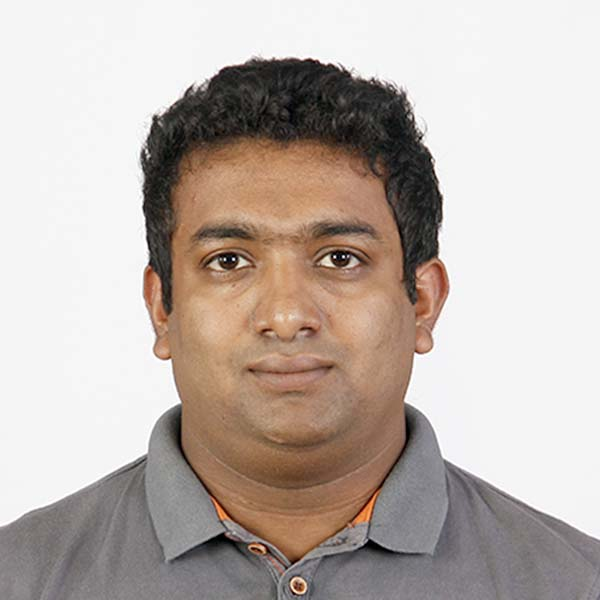
\includegraphics[scale=0.9]{img/photo.jpg}
    ~
  \header{Janitha}{Madushan}
      {Software Engineer}
   ~
  \section{Address}
    {\whitebodyfont No:04, "Sunhill,"\\
    Vajirapura,\\
    Nuwara-Eliya\\
    Sri-Lanka}
    ~
  \section{Phone}
    {\whitebodyfont +94 71 57 81 553\\
    +94 75 97 46 502}
    ~
  \section{Mail}
    \underline{\href{mailto:janithasen@gmail.com}{{\whitebodyfont janithasen@gmail.com}}}
    ~
  \section{Web}
  	\vspace{0.10cm}
    \underline{\href{https://www.linkedin.com/in/janithamadushan}{{\whitebodyfont linkedin}}}
    \\
	\vspace{0.10cm}
    \underline{\href{https://stackoverflow.com/story/jmadushan}{{\whitebodyfont stackoverflow}}}
	\\	
	\vspace{0.10cm}
    \underline{\href{https://github.com/janitham}{{\whitebodyfont github}}}
    ~
  \section{Langauges}
  	{\whitebodyfont Sinhaleese (Native)\\
    Engilsh}
    ~
  \section{Civil status}
    {\whitebodyfont Married}
  	~  
  \section{OS Preference}
    \asidelist{{\whitebodyfont Windows}}
    {\includegraphics[scale=0.30]{img/star.png}
    \includegraphics[scale=0.30]{img/star.png}
    \includegraphics[scale=0.30]{img/star.png}
    \includegraphics[scale=0.30]{img/star.png}
    \includegraphics[scale=0.30]{img/star.png}}
    \asidelist{\whitebodyfont{Linux}}
    {\includegraphics[scale=0.30]{img/star.png}
    \includegraphics[scale=0.30]{img/star.png}
    \includegraphics[scale=0.30]{img/star.png}
    \includegraphics[scale=0.30]{img/star_empty.png}
    \includegraphics[scale=0.30]{img/star_empty.png}}
    ~
  \section{Programming}
    \asidelist{{\whitebodyfont Java}}
    {\includegraphics[scale=0.30]{img/star.png}
    \includegraphics[scale=0.30]{img/star.png}
    \includegraphics[scale=0.30]{img/star.png}
    \includegraphics[scale=0.30]{img/star.png}
    \includegraphics[scale=0.30]{img/star_empty.png}}
    \asidelist{\whitebodyfont{C}}
    {\includegraphics[scale=0.30]{img/star.png}
    \includegraphics[scale=0.30]{img/star.png}
    \includegraphics[scale=0.30]{img/star.png}
    \includegraphics[scale=0.30]{img/star.png}
    \includegraphics[scale=0.30]{img/star_empty.png}}
    \asidelist{\whitebodyfont{Pyhon}}
    {\includegraphics[scale=0.30]{img/star.png}
    \includegraphics[scale=0.30]{img/star.png}
    \includegraphics[scale=0.30]{img/star.png}
    \includegraphics[scale=0.30]{img/star_empty.png}
    \includegraphics[scale=0.30]{img/star_empty.png}}
    \asidelist{\whitebodyfont{.NET}}
    {\includegraphics[scale=0.30]{img/star.png}
    \includegraphics[scale=0.30]{img/star.png}
    \includegraphics[scale=0.30]{img/star.png}
    \includegraphics[scale=0.30]{img/star_empty.png}
    \includegraphics[scale=0.30]{img/star_empty.png}}
    \asidelist{\whitebodyfont{PHP}}
    {\includegraphics[scale=0.30]{img/star.png}
    \includegraphics[scale=0.30]{img/star.png}
    \includegraphics[scale=0.30]{img/star.png}
    \includegraphics[scale=0.30]{img/star_empty.png}
    \includegraphics[scale=0.30]{img/star_empty.png}}
    ~
\end{aside}

\section{Experience}
\begin{entrylist}
  \entry
    {Nov. 15 - Now}
    {Software Developer}
    {Cambio Software Engineering}
    {I am working in automation team in configuration management team as a software developer. My responsibility 
    is to automate manual tasks in continuous delivery, continuous integration and management tools. On that tasks
    I developed various tools using various technologies. Mainly I developed tools using maven-plugins(MOJO), JAVA 
    and various technologies.}
  \entry
    {Oct. 15 - March.16}
    {Internship}
    {IFS R\&D}
    {I worked with "Technology" team and two distinct internal projects during my internship. I developed one internal
	application and a research project. In that period I exposed to ASP.NET, ORACLE 11G/12C, PLSQL, ANDROID and JAVA.}
\end{entrylist}

\section{Education}
\begin{entrylist}
  \entry
    {Aug. 11 - June 15}
    {Computer Engineering}
    {Faculty of Engineering, University of Peradeniya}
    {I followed computer engineering at Faculty of engineering of University of Peradeniya, Sri-Lanka. There I specified in 			 software engineering}
\end{entrylist}

\section{Projects}
\begin{entrylist}
  \entry
    {Oct. 16 - Now}
    {Package Automation tool(Continuous delivery)}
    {Stacker}
    {Stacker is continuous delivery automation tool. This works on fully mavenized environment. Stacker can be used as an JAVA 		application or as a maven plugin, it generates multi-module pom structure configured with different maven plugins(Two 			different frameworks are used in the product, those packaging in different orders, uses different plugins) using matadata(An artifact is released to nexus). Finally the package can be generated using the pom structure. This stacker is recently using as a maven plugin which is configured in a jenkins job, the job has also integrated with JIRA. Now the package requester 		can create the package him self. This has configured as a pipeline project in Jenkis job. Also a different phase is used in the pipeline with maven plugin to update package information management tool(Snooper) with its api.(Java, Maven-plugins,Jenkins, Jenkins-pipelines, Nexus, JIRA)}
    \entry
    {Aug. 15 - Oct. 15}
    {Packaging data management tool}
    {Snooper}
{This is a sub-project of package-automation(Stacker) project. An application was needed to store the packaging information. Snooper provides and restful-api and graphical user interface to do necessary operations.This snooper architecture is based on micro-services-architecture. It is used micro-service architectures with Spring Cloud and Docker.(Spring-cloud,Spring, hibernate, ms-sql, AngularJs, Java)}
\end{entrylist}

\newpage

\begin{aside}
\end{aside}

\begin{entrylist}
	\entry
    {June 15}
    {Device dependent CAPTHCHA System}
    {Final Year Project}
    {CAPTCHA system that provides suitable CAPTCHAs for suitable devices
	by  detecting  the  device,  then  provides  the  CAPTCHAs  as  their 
	functionalities and usability.}
  \entry
    {June 15}
    {IFS Rest Data service}
    {Internship Project}
    {Research on exposing database hosted server  APIs  as  RESTful  services. 
	Demonstrated  using  MS  excel  office  application}
  \entry
    {June 15}
    {IFS Day-Care Application}
    {Final Year Project}
    {Web  based  application  used  by  IFS  employees  to  reserve  the  day-care 
	facility at IFS. (Used ASP.NET, PLSQL, Oracle 11g database, Android, 
	Java)}  
  \entry
    {June 15}
    {Multi User Chat Room}
    {Systems \& Network Programming Lab}
    {Particular number of clients can be connected with the server. If any 
	client  sends  a  message, subsequently  the  massage  will be broadcasted to the other client. 
	(C, Socket programming, Multi-Threading)}
  \entry
    {June 15}
    {Tag Cloud}
    {Systems \& Network Programming Lab}
    {Get most frequent words from multiple HTML files which are in 
	multiple directories and creates a tag cloud out of those words using a 
	SVG. (C, Unix Shell Scripting, Multi-Processing )}
  \entry
    {June 15}
    {Microphone Alternator of Android}
    {Computer Engineering Project}
    {This system mainly has clients and main server application. The client requests to connect with the server application to 			uni-cast the sound stream. Subsequently, the client gets the access token to connect to server client can start uni-casting 			the sound stream (thorough smart-phones microphone). The server application plays the sound stream.  
    (Android, Java, UDP Socket Programming, multi-casting, uni-casting)}
\end{entrylist}

\vspace{3cm}

\begin{entrylist}
  \entry
    {}
    {}
    {}
    {References upon Request}
\end{entrylist}

\begin{entrylist}
  \entry
    {}
    {}
    {}
    {I do here by certify that above particulars are true and correct. If you are pleased to consider me 
	suitable for your company and select me as an employee, it will be my earnest endeavor to discharge 
	the duties entrusted to me, to the best of my ability and rise to your expectations.}
\end{entrylist}

\begin{flushright}
\emph{Janitha Madushan}
\end{flushright}
\begin{flushright}
\emph{\today}
\end{flushright}

\end{document}